\documentclass[convert=pdf2svg]{standalone}
\usepackage{tikz,pgfplots}
\usepackage{xcolor}

\renewcommand{\familydefault}{\sfdefault}

\usepackage{sansmath} % sans serif math                                                                                                                               
\sansmath % if you use it globaly                                                                                                                           

\usetikzlibrary{decorations.pathreplacing}

\begin{document}
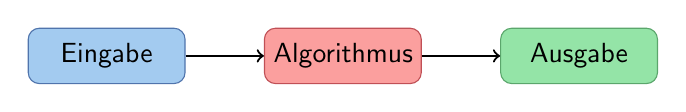
\begin{tikzpicture}[node distance = 3cm, auto, scale=3]

  \definecolor{my_blue}{RGB}{80,116,172}
  \definecolor{my_blue_light}{RGB}{163,203,240}
  \definecolor{my_orange}{RGB}{217,132,92}
  \definecolor{my_orange_light}{RGB}{251,180,139}
  \definecolor{my_green}{RGB}{91,166,108}
  \definecolor{my_green_light}{RGB}{148,228,167}
  \definecolor{my_red}{RGB}{192,80,86}
  \definecolor{my_red_light}{RGB}{251,159,158}	
  \definecolor{my_gray_dark}{RGB}{60,60,60}

  \tikzstyle{block} = [rectangle, draw, text width=5em, text centered, rounded corners, minimum height=2em]
  
%	\tikzstyle{every node}=[font=\fontsize{35}{0}\selectfont]
%	\tikzstyle{boxes_style}=[draw=border_color,fill=fill_color, line width=1.5mm]

  \node [block, draw=my_blue, fill=my_blue_light] (eingabe) {Eingabe};
  \node [block, draw=my_red, fill=my_red_light, right of=eingabe] (algorithmus) {Algorithmus};
  \node [block, draw=my_green, fill=my_green_light, right of=algorithmus] (ausgabe) {Ausgabe};

  \path [draw, thick, ->] (eingabe) -- (algorithmus);
  \path [draw, thick, ->] (algorithmus) -- (ausgabe);  

\end{tikzpicture}
\end{document}
